% Drawing a graph
% Author: Stefan Kottwitz
% https://www.packtpub.com/hardware-and-creative/latex-cookbook
\documentclass[border=10pt]{standalone}
\usepackage{tkz-graph}

\tikzset{
  LabelStyle/.style = { rectangle, rounded corners, draw,
                       font = \bfseries },
  EdgeStyle/.append style = {->} }
\thispagestyle{empty}
\begin{document}
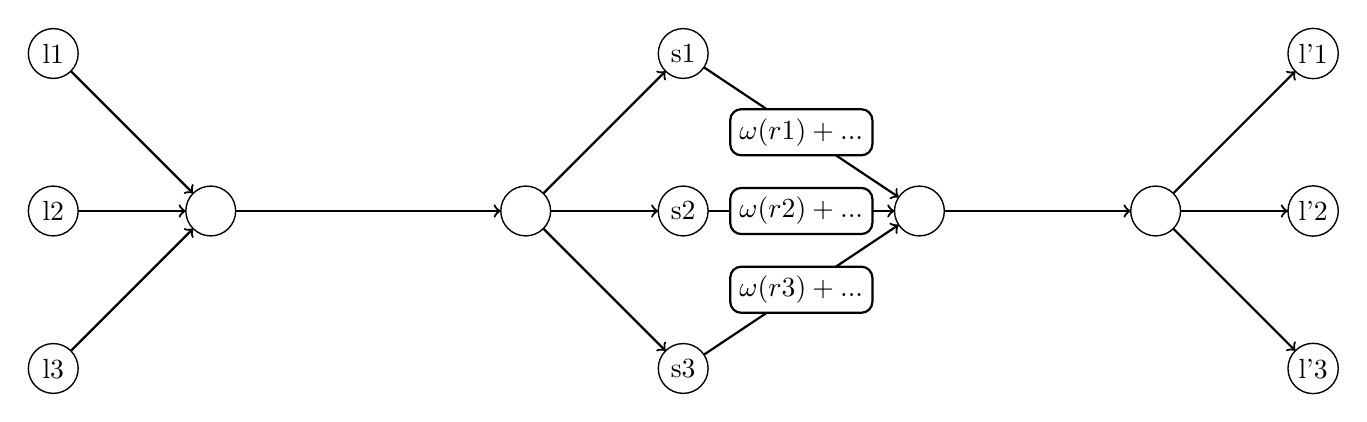
\begin{tikzpicture}
  \SetGraphUnit{5}
  \Vertex[x=0,y=0]{l3}
  \Vertex[x=0,y=2]{l2}
  \Vertex[x=0,y=4]{l1}
  
  \Vertex[x=8,y=0]{s3}
  \Vertex[x=8,y=2]{s2}
  \Vertex[x=8,y=4]{s1}
  
  \Vertex[x=16,y=0]{l'3}
  \Vertex[x=16,y=2]{l'2}
  \Vertex[x=16,y=4]{l'1}
  
  \SetVertexNoLabel
  \Vertex[x=2,y=2]{A}
  \Vertex[x=6,y=2]{B}
  
  \Vertex[x=11,y=2]{C}
  \Vertex[x=14,y=2]{D}
  
  \Edge(l1)(A)
  \Edge(l2)(A)
  \Edge(l3)(A)
  
  \Edge(B)(s1)
  \Edge(B)(s2)
  \Edge(B)(s3)
  
  \Edge(A)(B)

  \Edge[label = $\omega(r1)+...$](s1)(C)
  \Edge[label = $\omega(r2)+...$](s2)(C)
  \Edge[label = $\omega(r3)+...$](s3)(C)
  
  \Edge(D)(l'1)
  \Edge(D)(l'2)
  \Edge(D)(l'3)
  
  \Edge(C)(D)
\end{tikzpicture}

\end{document}